\chapter{Projektplanlægning}\label{Projektplanlaegning}
Dette kapitel vil afbilde hvordan gruppen har planlagt projektforløbet både tidsmæssigt samt opgavemæssigt, og hvilke redskaber som er blevet anvendt af gruppen undervejs til at håndtere planlægningen igennem processen. Planlægningen er en af de væsentligste aspekter til at sikre sig, at det er muligt at overholde projektets deadlines, samt at sikre sig at alt kan nå at blive færdiggjort. Såfremt det ikke er muligt at holde en deadline, eller at den bliver færdiggjort før tid, har det været nødvendigt at tage den gældende kalenderen op til revidering og tilpasse den, således at der kan skabes et nyt overblik hvor langt foran eller bagud projektet er henne tidsmæssigt. Til slut vil der blive reflekteret over projektplanlægningen som helhed har fungeret.

\section{Tids- og opgaveplanlægning}\label{Tidsplanlaegning}
For at optimere arbejdsprocessen bedst muligt og udnytte den afsatte tid til projektet på optimalt vis, blev det besluttet i gruppen at der skulle udarbejdes en form for tidsplanlægning. Dette skulle laves på både dags-, uge- og månedsbasis for at skabe et overblik over hvordan tiden skulle bruges, samt for at sikre at alle gruppens medlemmer altid havde noget at gå i gang med, såfremt nogen manglede noget at lave. Til dette blev det besluttet at benytte forskellige redskaber som dagsorden, Trello og Gantt-diagram, som havde hvert deres formål. For at dette skulle fungere, krævede det dog at alle redskaberne spillede sammen med hinanden, således at de alle pegede i samme retning, da de ellers ville være mere vildledende end til gavn for gruppen.

\subsection*{Gantt-diagram}\label{Gantt-diagram}
Efter den første måned af projektarbejdet, som primært bestod af materiale søgning og idéudvikling sidelæns med reeksamen, blev der udviklet et Gantt-diagram. Det havde til formål at give et overblik på uge- og månedsbasis, over hvordan gruppen forventede at tiden ville blive brugt på de forskellige dele som rapporten skulle indeholde. Gantt-diagrammet var tiltænkt at give et estimat over hvordan projektet skulle struktureres, men ikke til at give et overblik over alle de små underopgaver, som hvert tiltænkt afsnit skulle indeholde eller fordeles imellem gruppens medlemmer. Det første Gantt-diagrammet som blev udviklet, skulle benyttes som en indikator for hvordan gruppen mente tiden skulle fordeles på de forskellige dele af projektet, som hvad flertallet mente var mængden af tid der skulle afsættes til det. Alle var dog indforstået med at der undervejs skulle ændres på det, eftersom at nogle ting højest sandsynligvis ville tage længere eller kortere tid end forventet.

\begin{figure}[h]
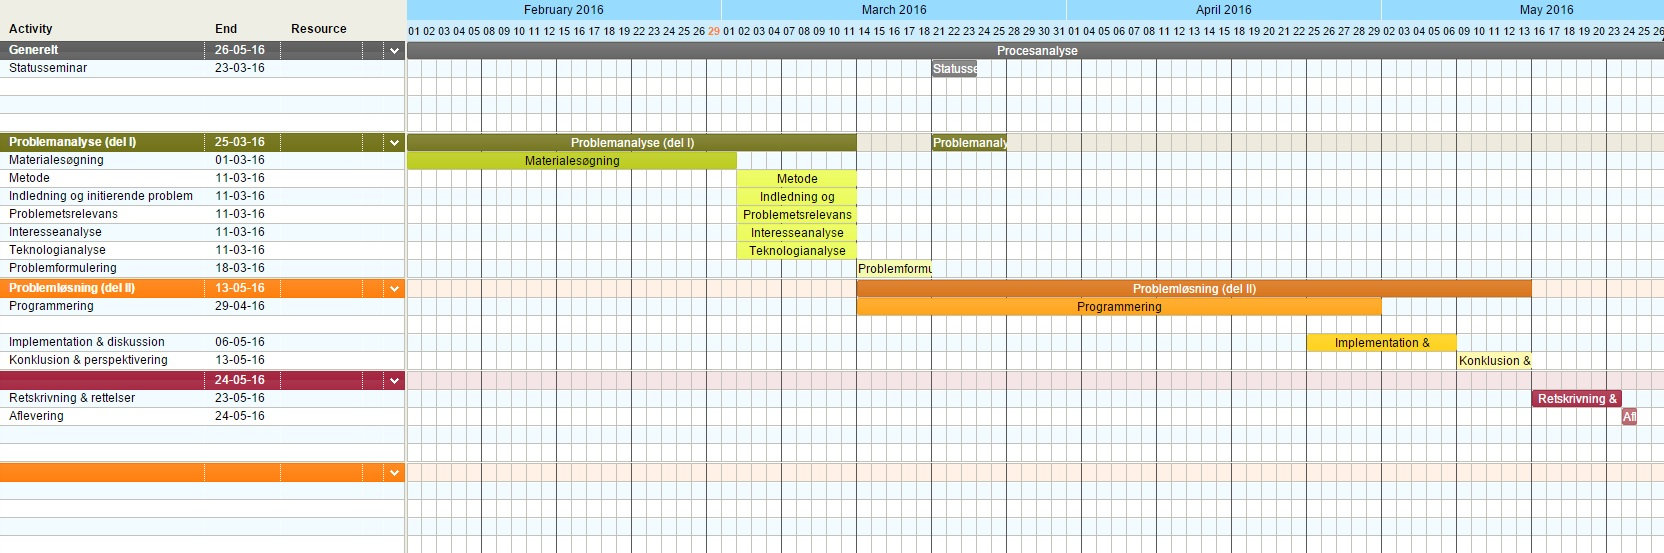
\includegraphics[scale=0.35]{SimuleringGanttdiagramStart}
\centering
\caption{Gruppens første gantt-diagram}\label{Gantt-diagram-picture}
\end{figure}

Herefter var det så meningen, at det skulle ændres på hver gang ugen var omme til fredagsmøderne, således at det kunne tages op til en revidering og få et bedre overblik hvor langt foran eller bagud gruppen var med projektet. Gantt-diagrammet vil på den altid være up-to-date med hvor langt gruppen var kommet i projektet, og kunne bruges som en motiverende faktor til at se hvor langt vi var nået i forhold til forrige uge.

\begin{figure}[h]
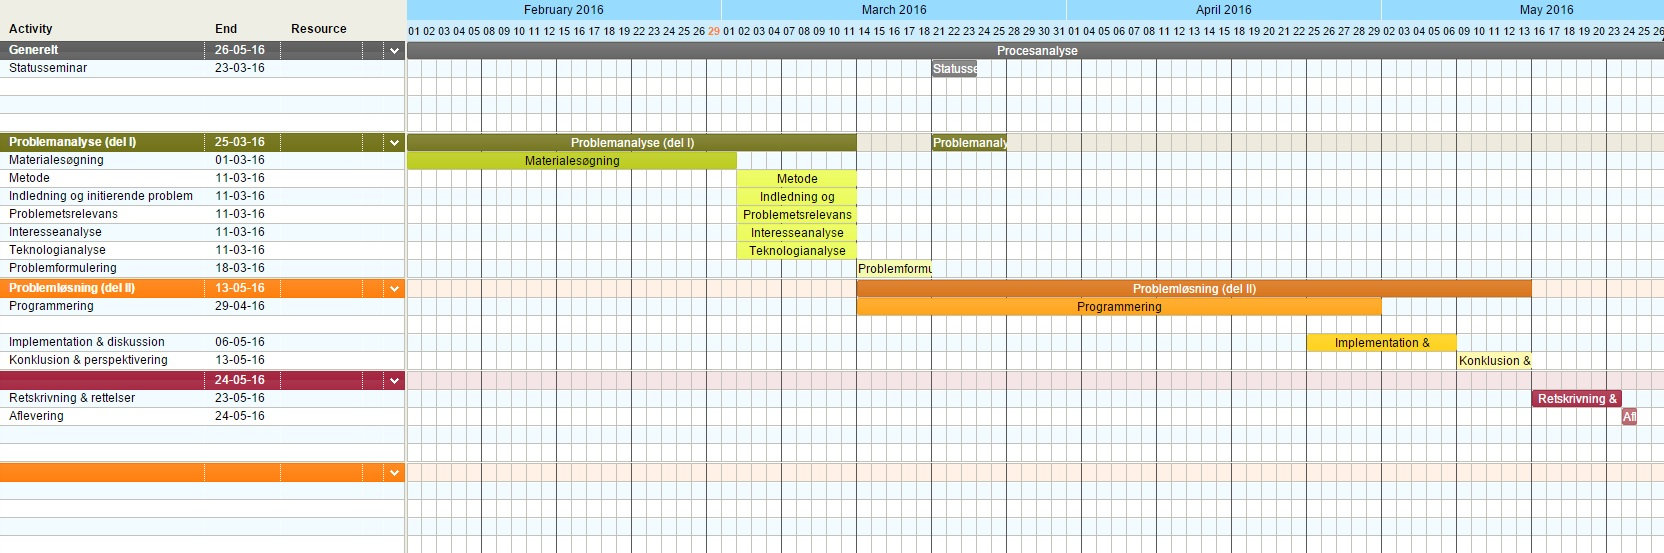
\includegraphics[scale=0.35]{SimuleringGanttdiagramStart}
\centering
\caption{Gruppens gantt-diagram efter sidste revidering}\label{Gantt-diagram-picture}
\end{figure}

\subsection*{Dagsorden}\label{Dagsorden}
Indledende til projektarbejdsdage blev der benyttet en dagsorden på tavlen, hvor det arbejde som var blevet lavet siden sidst blev diskuteret, samt om der var opstået nye punkter som yderligere skulle tilføjes til opgaver siden sidst. Alle havde til opgave at læse det nye materiale der var blevet skrevet siden sidst, så hvis der var noget der skulle diskuteres. Dagsorden blev kun systematisk anvendt hver tirsdag eller på dage hvor der ikke var nogen forelæsninger, ellers blev den kun anvendt, hvis der var et eller flere gruppemedlemmer som ikke vidst hvad de skulle gå i gang med. 

dagsorden blev brugt til at finde ud af hvad der skulle laves og hvad der skulle tilføjes til Trello, mens Trello blev brugt til at holde styr om opgaverne blev lavet og hvilket medlem eller medlemmer af gruppen der sad på de forskellige opgaver.

\begin{figure}[h]
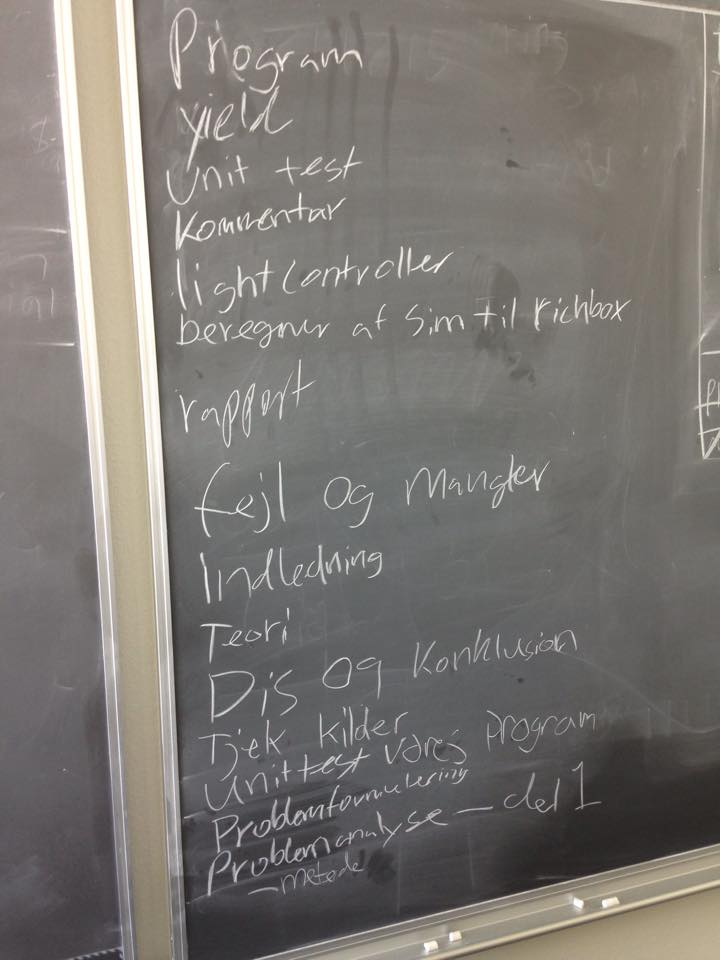
\includegraphics[scale=0.35]{Dagsorden}
\centering
\caption{Et udsnit af en typisk dagorden fra gruppens tavle}\label{Dagsorden}
\end{figure}


En typisk dagsorden for gruppen kunne se ud som vist ovenstående. Den blev ikke skrevet op på en systematisk måde, eftersom alt alligevel ville blive overført til Trello efterfølgende, hvor det vil blive skrevet op systematisk med et mere overskueligt overblik.

\subsection*{Trello}\label{Trello}
Trello er en hjemmeside som tilbyder brugerer muligheden for at oprette grupperum hvori man kan oprette opgaver og sætte disse opgaver under forskellige katagorier. Denne type opsætning er baseret på-, samt opfordret til, at følge scrum udviklingsmetoden. Scrum handler om projektledelse og deligeringen af arbejdsopgaver. Scrum er et meget frit og meget velkendt model inde for software udvikling.

Trello blev brugt som en tilbygning til dagsorden og havde nogenlunde samme formål. Alt der blev opskrevet på dagsorden blev tilføjet i Trello, således at det var på et elektronisk medie alle havde adgang til, hvortil hver opgave blev opdelt i underopgaver der skulle udføres. Efterfølgende var det så muligt at tilføje andre og sig selv til forskellige opgaver, hvor det således var muligt at afkrydse når en opgave eller underopgave var færdiggjort, eller tilføje flere  opgaver eller underopgaver, hvis der var behov for det. Dette gjorde det muligt for folk at se hvad der blev lavet, hvem der gjorde det og hvornår det skulle være færdigt, selv hvis man ikke havde været der den pågældende dag. Dette gjorde også at man bare kunne hoppe videre med en ny opgave, såfremt man skulle blive færdig med ens eget før andre. Det var også en hjælp til at opdage, hvis der var nogle punkter som lød meget ensformigt der kunne slås sammen, eller om det var det samme to skrev om eller to vidt forskellige ting, så man kun orientere sig med gruppen om det. 

\begin{figure}[h]
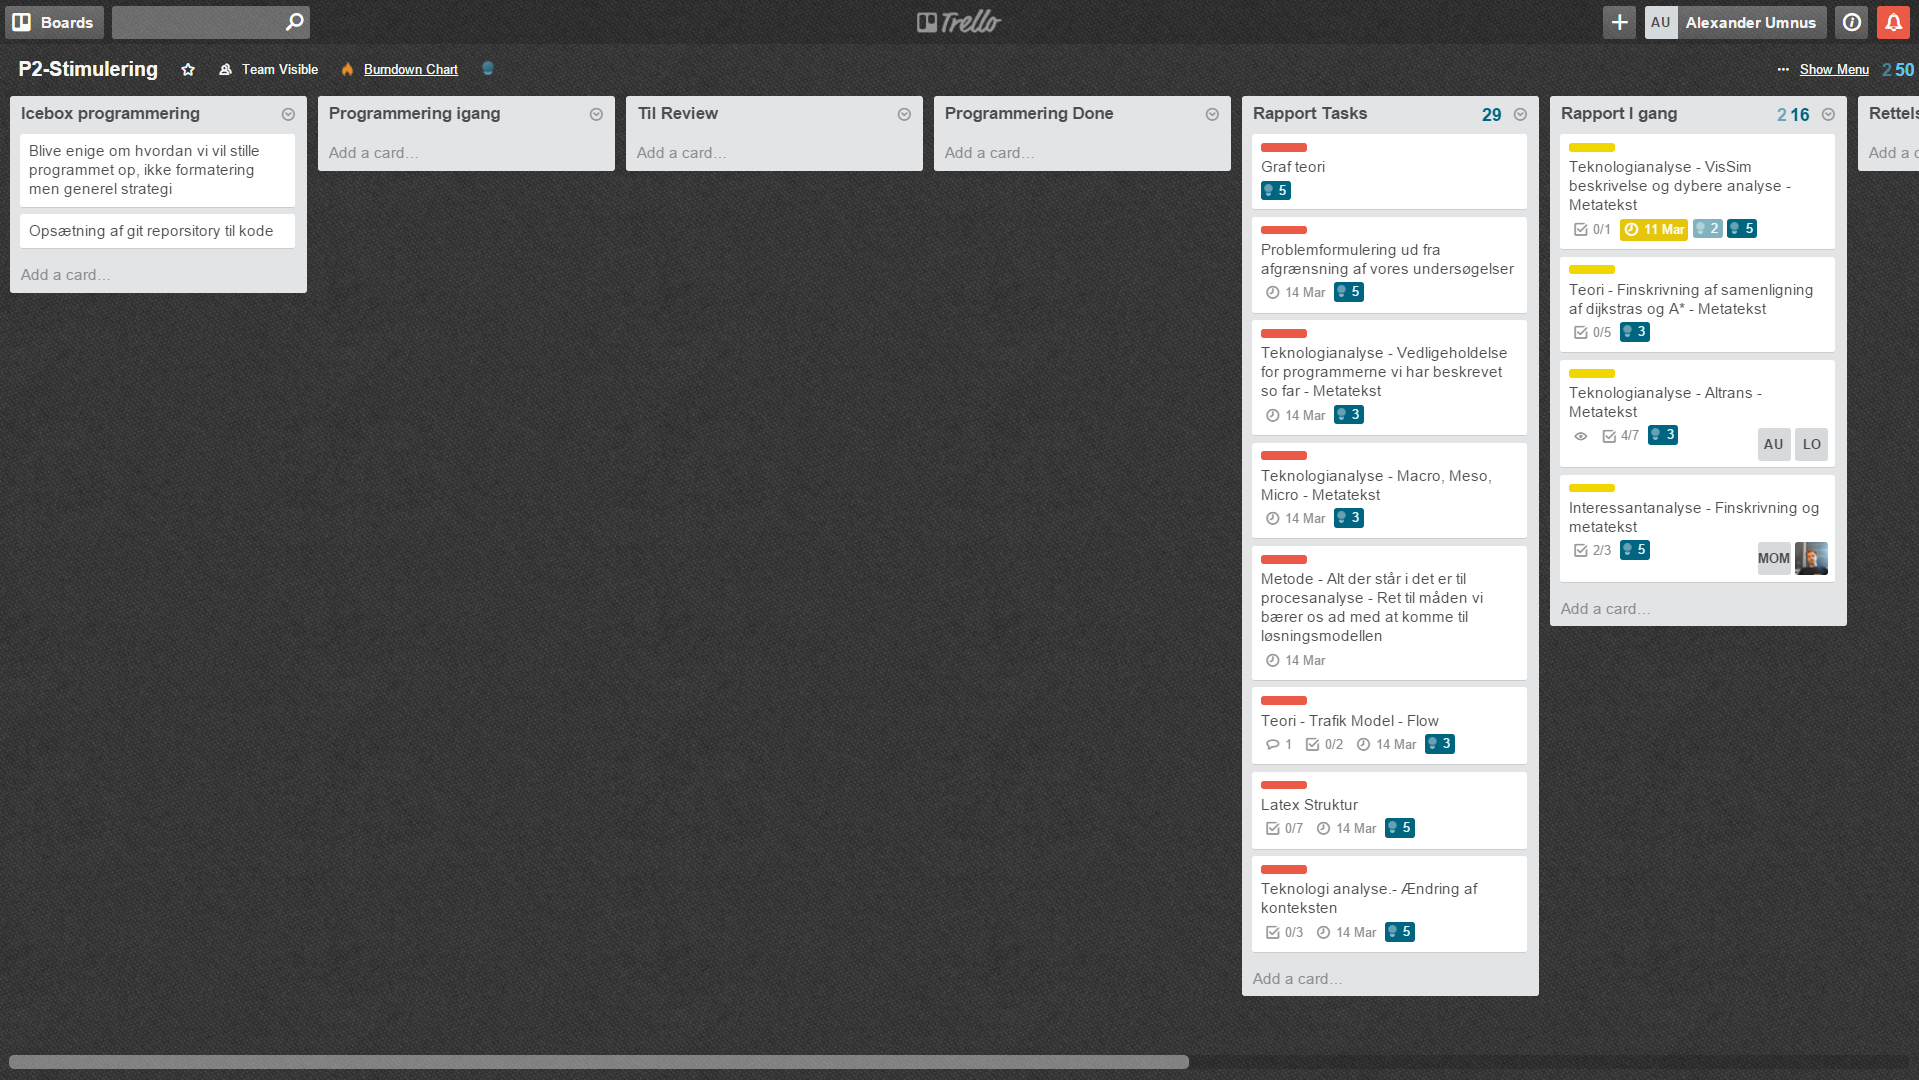
\includegraphics[scale=0.25]{figures/Trello1}
\centering
\caption{Et udsnit af gruppens Trello}\label{Trello}
\end{figure}

Et udklip af hvordan gruppens Trello endte med at se ud efter projektet var overstået kan ses på ovenstående billede. Opgaverne blev inddelt i punkterne, "rapport task", "rapport i gang", "rettelser" og "rapport done", som så kunne flyttes ind i de forskellige rubrikker alt efter hvor i processen de var. Når en opgave blev lavet blev den tildelt enten "rapport task" eller "rapport i gang" eller efter om der var tildelt et gruppemedlem på forhånd eller ej, hvorefter det så vil blive flyttet over i enten "rapport rettelser" eller "rapport done" alt efter om nogen mente noget skulle rettet, eller om det var som det skulle være og færdiggjort. I de fleste tilfælde ville gruppen arkiverer opgaver der var færdige således at vi kun havde de nyeste og relevante opgaver på selve trello skemaet.

\section{Reflektion over projektplanlægningen}\label{Reflektion-over-projektplanlaegningen}
I startfasen blev alle de forskellige redskaber sat op og klar til brug. Det var meningen at de skulle benyttes men de blev desværre sat i bero under vores materialesøgning og idéudvikling da gruppen brugte meget tid på at læse og ideudvikle. Gruppen har dog været nødt til at erkende at projektplanlægningen ikke har været optimal, selvom der blev lagt hårdt ud fra start med hvordan det skulle organiseres, men begyndte så småt som projektet skred frem at forsømme det som aftalt. På trods af at gruppen var enige om at opretholde et ganttdiagram for at holde styr på langtsigtede planlægning, blev dette ikke overholdt mere end et par uger. Dette har på sin vis ikke gjort de største skader på projektarbejdet da opgaver der skulle løses blev sat ind på trello istedet med deadlines til hvornår disse skulle være løst. Den største ulempe ved ikke at holde ganttdiagramet har været at have et overblik over projektet samt manglen på langsigtet planlægning. Derudover har gruppen ikke været gode til at opretholde brugen af Slack, det var meningen at gruppen ville bruge Slack til at holde styr på arbejdsrelateret emner som blev diskuterert online og udenfor grupperummet, men da der ikke blev diskuteret meget ud over mødetider, ophørte brugen af Slack inde for et par uger. Derimod blev arbejdsrelateret emner på et senere tidspunkt diskuteret over VoIP programet kaldt Discord\ref{Gruppekommunikation}.